\documentclass[acmsmall,screen,anonymous]{acmart} % remove review to delete lines

\title[\ours]{\ours: Interactive Query-Oriented Text Analytics for Comprehensive Investigation of Historical News Archives}

\newcount\Comments  % 0 suppresses notes to selves in text
\Comments=1   % TODO: set to 0 for final version


%% 
\newcommand{\deltaCQengaged}{0.519} % the difference in means between CQ and IR. Comes from deltaCQengaged.txt
\newcommand{\deltaCQall}{$0.399$}

% computed in histogram_maker.R
\newcommand{\cohensengaged}{0.495} % d_engaged.txt
\newcommand{\cohensALL}{0.352}  % d_all.txt
\newcommand{\nengaged}{62} 
\newcommand{\nengagedIR}{32}
\newcommand{\nengagedCQ}{30}
\newcommand{\cqNperfectscore}{8}
\newcommand{\irNperfectscore}{4}
\newcommand{\pAll}{0.030} % p_all.txt
\newcommand{\pAttentive}{0.029} % p_attentive.txt

% these numbers are reported in the table reporting user study
\newcommand{\totalNmin}{40.3} % this number is (121 workers * 20 min/worker)/(60 min/hr), rounded to .3
\newcommand{\totalN}{121} % totalN.txt

%%%


% for comments
\usepackage{color}

\usepackage{tikz}
\definecolor{CCPurple}{rgb}{.405, .144, .450} % hex 672573
\definecolor{darkgreen}{rgb}{.106, .471, .216}
\definecolor{gold}{RGB}{240,205,17}

%% Notation 
\newcommand{\Q}{$Q$}
\newcommand{\mentions}{$\mathcal{M}(\Q)$} % from police fatalities 
\newcommand{\queryresponsivedocs}{$\mathcal{D}_\Q$} % from police fatalities
\newcommand{\specificmention}{$i \in \mathcal{M}(Q)$} % from police fatalities 
\newcommand{\newsstory}{$d$} % from manning IR book table of notation 
\newcommand{\timestamp}{$t$} % from manning IR book table of notation  https://nlp.stanford.edu/IR-book/pdf/irbookonlinereading.pdf
\newcommand{\doctimestamppair}{$(d, t)$}
\newcommand{\archive}{$\mathcal{A}$} % an archive, = [(d_0, t_0), (d_1, t_1) ... (d_N, t_N)]
\newcommand{\mentionincontext}{$\mathcal{C}(i)$}
\newcommand{\simplifiedsentence}{ $\mathcal{C}_{s^{\prime}}(i)$}



\newcommand{\kibitz}[2]{\ifnum\Comments=1\textcolor{#1}{#2}\fi}
%\newcommand{\abe}[1]{\kibitz{red}{[Abe: #1]}}
%\newcommand{\nm}[1]{\kibitz{blue}{[NM: #1]}}
%\newcommand{\bto}[1]{\kibitz{darkgreen}{[BTO: #1]}}
\newcommand{\ione}{I1}
\newcommand{\itwo}{I2}
\newcommand{\ithree}{I3}
\newcommand{\ifour}{I4}
\newcommand{\ifive}{I5}
\newcommand{\rhone}{H1}
\newcommand{\rhtwo}{H2}
\newcommand{\ours}{\textsc{ClioQuery}}
\newcommand{\R}{skimmable mentions}
\newcommand{\burdensome}{mention gathering}
\newcommand{\sshot}[1]{\includegraphics[height=4cm]{#1}}
\newcommand{\Strategy}{Pattern}
\newcommand{\pattern}{pattern}
\newcommand{\Strategies}{Patterns}
\newcommand{\patternsLong}{design patterns}
\newcommand{\PatternsLong}{Design patterns}
\newcommand{\designpatterns}{design patterns}
\newcommand{\designpatternsshort}{strategies}
\newcommand{\titleoffset}{-3cm}
\newcommand{\captionname}[1]{\hspace*{.1cm} #1}
\newcommand{\roverview}{R1}
\newcommand{\rcomprehensive}{R2}
\newcommand{\rcontext}{R3}
\newcommand{\rnoconfound}{R4}
\newcommand{\rmax}{R4}
\newcommand{\appendixwidth}{width=7cm}
\newcommand{\Baselongname}{keyword document search}
\newcommand{\BaselongnameCap}{Keyword document search}
\newcommand{\marginwidth}{.1} % min w/o word wrap
\newcommand{\cellwidth}{.28}
\newcommand{\includewidthFam}{.9}
\newcommand{\lastletter}{I}
\newcommand{\leftwidth}{1.9cm}
\newcommand{\familypicwidth}{3.9cm}
\newcommand{\familypicwidthPlus}{5.5cm}

\usepackage{multirow}
\usepackage{makecell}
\usepackage{subcaption}
\usepackage{bm}
\usepackage{enumitem}
\usepackage[normalem]{ulem} 

\usepackage{cleveref} % needed to ref a footnote in Sys section
% https://tex.stackexchange.com/questions/167380/how-to-refer-to-a-footnote


%%
%% \BibTeX command to typeset BibTeX logo in the docs
\AtBeginDocument{%
  \providecommand\BibTeX{{%
    \normalfont B\kern-0.5em{\scshape i\kern-0.25em b}\kern-0.8em\TeX}}}

%% Rights management information.  This information is sent to you
%% when you complete the rights form.  These commands have SAMPLE
%% values in them; it is your responsibility as an author to replace
%% the commands and values with those provided to you when you
%% complete the rights form.
\setcopyright{acmcopyright}
\copyrightyear{2021}
\acmYear{2021}
\acmDOI{xxx}


%%
%% These commands are for a JOURNAL article.
\acmJournal{TIIS}
\acmVolume{xx}
\acmNumber{xx}
\acmArticle{ACM Article No}
\acmMonth{1}

\begin{document}

%%
%% If your work has an appendix, this is the place to put it.
\appendix


\section{Appendix}
\subsection*{The \ours~system: additional details}


\subsubsection*{Implementation details}
\ours~is a web application written in Python 3, using the Flask and React libraries.\footnote{\url{https://flask.palletsprojects.com/en/1.1.x/} and \url{https://reactjs.org/}} The text simplification methods in the paper use Stanford CoreNLP \cite{corenlppipeline} for tokenization, dependency parsing, and part-of-speech tagging.\footnote{Eisenstein \cite{eisenstein2019introduction} offers a detailed introduction to these NLP techniques.}  \ours's relationship span extraction method also employs logistic regression; we use the implementation from Scikit-learn \cite{Pedregosa:2011:SML:1953048.2078195}.
In the future, rewriting our Python-based prototype~in a faster language like Java or C would reduce our system's latency, helping \ours~scale to larger corpora.
It might also be possible to further improve performance by employing time and space efficient IR methods for efficiently indexing and retrieving the locations of query words in documents \cite{irbook}.

\subsubsection*{Time Series View: additional details}
\ours's {Time Series View} shows a single rug point (small vertical line) for each document mentioning the query.
These markings both help explain aggregated count statistics encoded in the time series plot (more rug points mean an higher annual count), and help link the Time Series View with the Document Feed. 
If a user hovers over a rug point, \ours~displays the headline of the corresponding news story using a tooltip; if the user clicks a rug point, \ours~updates so that the story is displayed in the Document Feed and in the Document Viewer.
When a user hovers over some year in the Time Series View, \ours~displays a tooltip showing the total count of documents containing the query for that year.

\subsubsection*{Default system behaviors}
If a user has not yet entered a query, \ours's time series plot simply shows the overall counts of documents by year across the entire corpus, shown with a neutral black line.
In this case, the Document Feed also shows all documents in the corpus. Moreover, when filter-by-date is not used, \ours~shows documents from the time span of the corpus.

\subsubsection*{Choosing colors}
We {chose colors for \ours} using Colorbrewer \cite{colorbrewer}, a common resource, which offers colorblind safe and print-friendly palettes.
Hall and Hanna \cite{HallAndHanna} test how foreground and background color affects how people read, retain, and experience text on screen. Our study focuses on testing the utility of in-text highlighting and text simplification for expert social researchers; future work might test the effect of varying the foreground or background color.

\subsubsection*{Handling token gaps during clause deletion}
In some cases, there may be gaps between tokens in simplified mentions, where tokens have been removed from the middle of a sentence. 
(These are shown with ellipses in the Document Feed).
In these cases, in performing {automatic in-text highlighting to link the Document Feed and Document Viewer}, we highlight the span in the Document Viewer which begins with and ends with the first and last token of the corresponding simplified mention, shown in the Document Feed.

\subsubsection*{Computing tf-idf scores of iterative clause deletion}
To compute tf-idf scores during iterative clause deletion, we assign each word in each possible output candidate shortening a word-level tf-idf score, and average the word-level tf-idf scores of all words in each possible candidate shortening to compute an overall, sentence-level tf-idf score. 
We assign each word a tf score equal to the total occurrences of the word among all documents that contain $Q$, and an idf score equal to 1 divided by the count of documents containing the word across the corpus.
We then multiply each word's tf score by its idf score to get a word-level td-idf score.
We then select the candidate shortening with the highest overall tf-idf score for display in the Document Feed.

\subsubsection*{Choosing among possible sentence shortening methods}
In the System section, we describe three different sentence shortening techniques, which are applied in the \ours~interface. 
Below, we describe how \ours~chooses to apply the three different methods.

After a user enters a query $Q$, for each document mentioning $Q$, \ours's Document Feed displays the first sentence within the document mentioning $Q$ that can be shortened via query-focused clause deletion.
If no such sentence exists, \ours~resorts to shortening the first sentence mentioning $Q$ via {character windowing}. 
(Character windowing is only used as a last resort because it does not attempt to create well-formed output containing salient words from the input.)

In cases when a user has entered both a query and subquery, for each document mentioning the query or subquery, \ours~will attempt to display the first sentence in the document that can be shorted via relationship span extraction.
This is because we assume the user is interested in the relationship between the query and subquery.
If there is no sentence that can be shortened via relationship span extraction, \ours~will display the first sentence that can be shortened via query-focused clause deletion.
If no sentence can be shortened via clause deletion, it will resort to shortening the first sentence mentioning the query or subquery via character windowing.


\ours~also allows the user to click ``expand'' to see all sentences mentioning the query within the document, as described in the System section. 
In this case, \ours~will first attempt to shorten each sentence mentioning $Q$ via query-focused clause deletion, before resorting to shortening the sentence with character windowing. 
If the user has also set a subquery (in addition to $Q$), \ours~will first try to shorten each sentence mentioning the query and subquery using relationship span extraction (and then attempt clause deletion, and character windowing).
\subsection*{Field study: additional details}

To help $H1$ answer their question using \ours, we gathered a custom corpus of articles from \textit{The New York Times} (NYT). To gather the corpus, we searched for ``El Salvador'' on \textit{The New York Times} website \cite{nytwebsite}, and then automatically downloaded all query-matching articles published between 1980 and 1985 in the World News and Week in Review sections of the newspaper. 
We filtered downloaded articles to create a corpus of NYT articles containing the word ``Salvador,'' and we loaded this corpus into \ours~for $H1$. 

To help $H2$ answer their research question, we similarly gathered a second custom corpus of articles by searching for ``astronaut'' on the \textit{New York Times} website \cite{nytwebsite}, and then automatically downloading all query-matching articles published between 1980 and 1985. We then similarly filtered the documents to ensure that all query-matching mentioned ``astronaut'' and loaded the corpus into \ours~for $H2$.
\subsection*{Quantitative comparison study: additional details}

\subsubsection*{Additional details regarding creation of reading comprehension questions}
We used a semi-automated procedure to create reading comprehension questions for our quantitative crowd study.
Specifically, we first collected all editorials from The New York Times Annotated Corpus \cite{SandhausNYT} which included the words ``Zimbabwe'' and ``Mugabe''.
We then used the TfidfVectorizer class from scikit-learn \cite{Pedregosa:2011:SML:1953048.2078195} with default settings to construct tf-idf vectors for all 1,689 sentences in the editorials. 
We also similarly constructed tf-idf vectors for all 597 sentences from the Wikipedia page on Robert Mugabe \cite{wikimugabe}. 
We then computed the cosine similarity of each sentence pair in the Cartesian product of Wikipedia and \textit{New York Times} sentences. We manually reviewed the 200 sentence pairs with the highest cosine similarities, and manually labeled 37 total sentences from \textit{New York Times} editorials which reported a fact described in some sentence from Wikipedia.
This process identified 37 facts about Mugabe from Wikipedia reported in editorials in \textit{The New York Times}. 
We selected 8 of these facts to create reading comprehension questions for our task.

% to make the file use mugabe tf-idf.ipynb
% replication cat mugabe.wiki.jsonl| grep -v wikipedia | wc -l => 1689
% cat mugabe.wiki.jsonl| grep wikipedia | wc -l

% Google sheet for this is Wikipedia linker. Countif on recall column gets the 37 facts

\subsubsection*{Additional details regarding tuning of IR baseline}
We implemented the IR baseline using Whoosh, an open-source Python search engine. Like many search engines, Whoosh shows small document snippets from ranked documents on the search engine results page (Figure \ref{f:appendix_ir_serp}). To encourage fair comparison between Whoosh and \ours, we tuned Whoosh so that document snippets contained roughly as much text as the shortened sentences in the \ours~Document Feed. 
Specifically, Whoosh allows snippet customization by setting the \texttt{maxchars} and \texttt{surround} parameters in its \texttt{Highlighter} module.
We set these parameters by performing a grid search over all possible values from 10 to 100 (for each parameter), in order to maximize the average number of characters per Whoosh document snippet, under the constraint that the average was less than or equal to 90 characters (the length of the longest-possible shortened sentence in the \ours~Document Feed).
The final setting for the \texttt{surround} parameter was 27 characters and the final setting for the \texttt{maxchars} parameter was of 10 characters. Using these settings, we observe a mean snippet length of exactly 90 characters using the IR system on the crowd task.
Beyond tuning these parameters, we use default settings for the Whoosh search engine.

\subsubsection*{Additional details regarding the crowd study pretest}
Before beginning the main task in our crowd study, participants in each condition used their interface to complete a three minute pretest using a small corpus of six \textit{New York Times} editorials mentioning ``Iraq''. 
The pretest was very similar to the main task; each interface was hard-coded to use the query ``Falluja'' and 
participants were instructed to ``find and remember everything the \textit{New York Times} wrote about Falluja'' using their tool.
After participants typed this exact phase into a text box to confirm they understood the instructions, they conducted research using their assigned interface.
After 3 minutes, participants were then presented with a screen with four facts about U.S.\ involvement in Falluja (included in supplemental materials),
and asked to identify which facts were reported in the six articles.
Because only one fact from the list was reported in the articles, 
to get a perfect score of 4 out of 4 on the pretest, workers had to both correctly identify the reported fact, and refrain from guessing any of the other three facts. 
The pretest was designed to be very easy for attentive workers.

\subsubsection*{Additional details regarding data collection phases for the crowd task}
Data collection for the crowd task proceeded in two phases: an initial pilot phase and a main data collection phase.
After the small pilot, we added two training screens for \ours~participants (shown in supplemental materials) to help \ours~users gain practice using unfamiliar features. 
We also fixed a bug in the pilot in which \ours~users were shown an extra two editorials. 
We emphasize that these two editorials did not contain any facts about Mugabe which could be used to answer the reading comprehension questions, and also note that the 
two extra editorials would have made the task harder for \ours~participants (because they would have had to read extra text during the task, which was not relevant to the reading comprehension questions).
Finally, after the pilot, we adjusted the random assignment mechanism so that participants were assigned to conditions in an alternating fashion following an initial random draw (i.e.\ first \ours, then IR, then \ours...). In the pilot, participants were assigned to conditions at random when they loaded the first screen in the task.

\subsubsection*{Additional details regarding task payment}
Because we had trouble recruiting qualified masters workers for our lengthy and complex task we increased payment during data collection. The first 18 participants were paid \$2.50 to complete the pilot. After the pilot, we increased payment to \$3.00 and collected data from 75 more participants. Because data collection was still very slow (e.g.\ 10 workers over a 24 hour period) we further increased payment to \$4.00 for the task and collected data from 26 more workers. Finally, we increased payment to \$5.00 for the task. When only 2 workers signed up over a half-day period at the \$5.00 rate we ended data collection.



\clearpage
\subsection{Additional Figures}

\begin{figure}[h]
\fbox{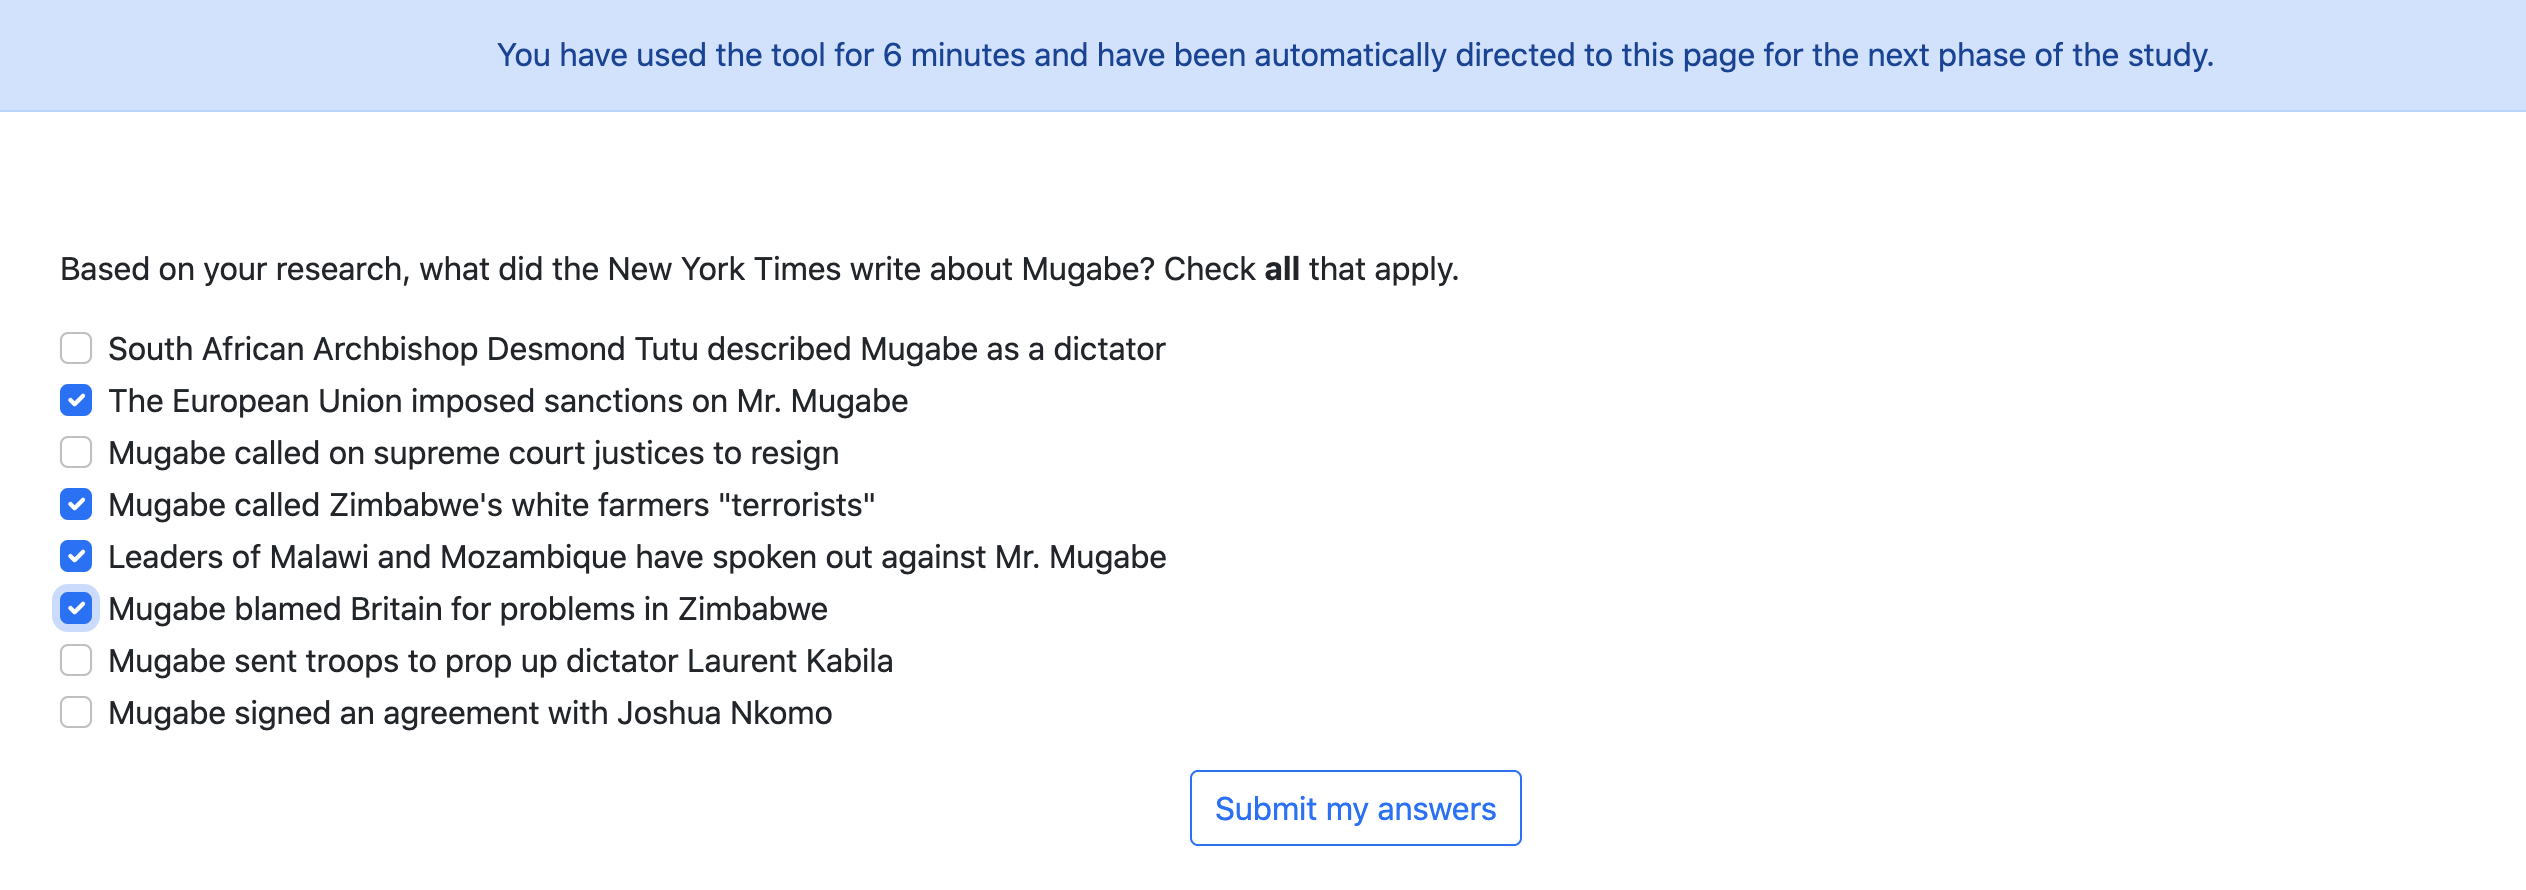
\includegraphics[width=14cm]{samples/appendix/MugabeQ.png}}
\caption{Participants answered eight true/false questions about what \textit{The New York Times} wrote about Robert Mugabe, using the form shown above. The four facts shown with checkboxes were described in editorials available to participants during the study. 
The four false facts shown without checkboxes were described in other editorials, not available to participants during the study. 
Participants who found and remembered the four facts from the corpus and who also did not incorrectly guess any of the four facts not described in the corpus scored 8 out of 8 on the reading comprehension task.
The order of questions was randomized.}
\end{figure}


\begin{figure}[h]
\fbox{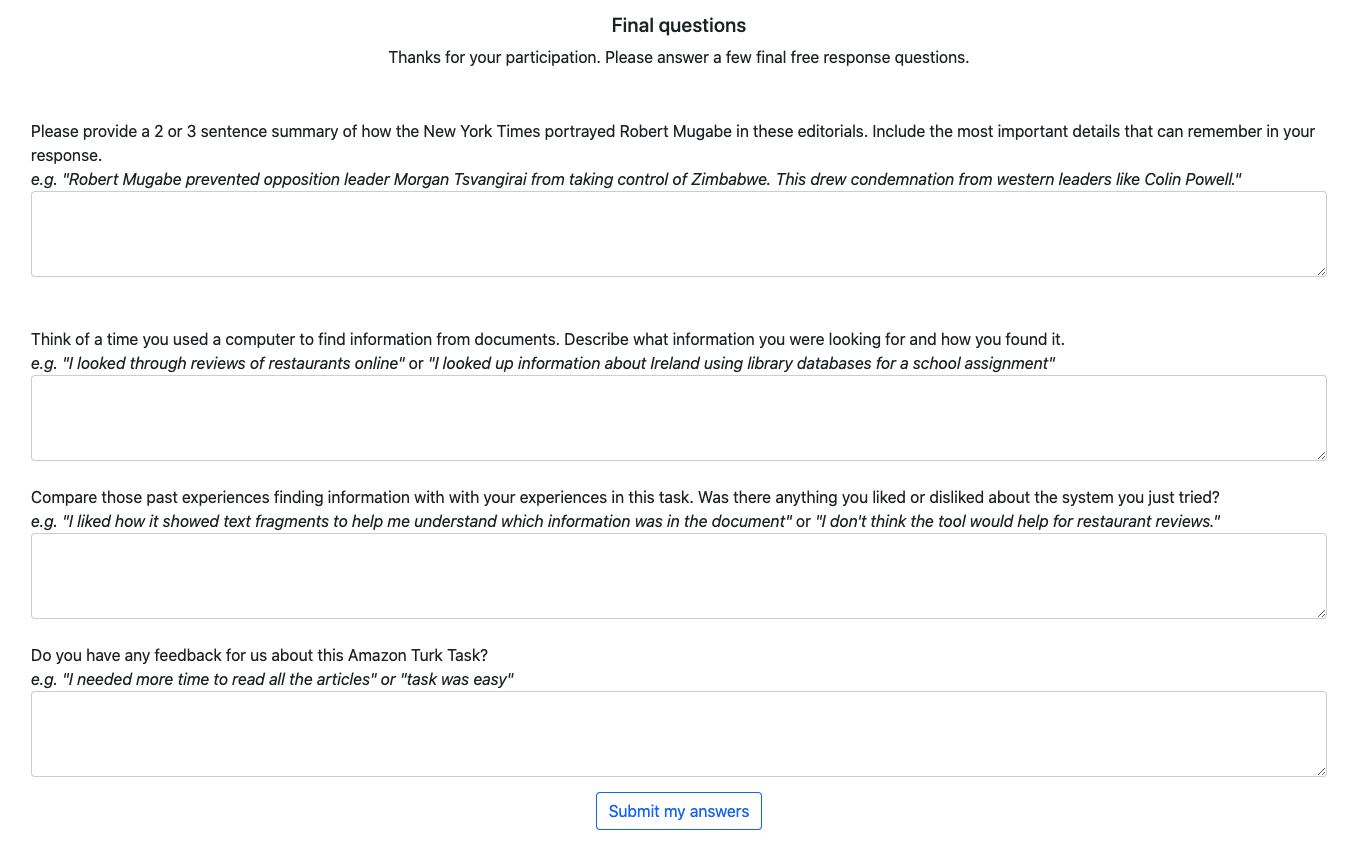
\includegraphics[width=14cm]{figures/qualQ.png}}
\caption{Qualitative questions for participants at the end of the crowd task}
\end{figure}


\begin{figure}[t!]
\centering
\fbox{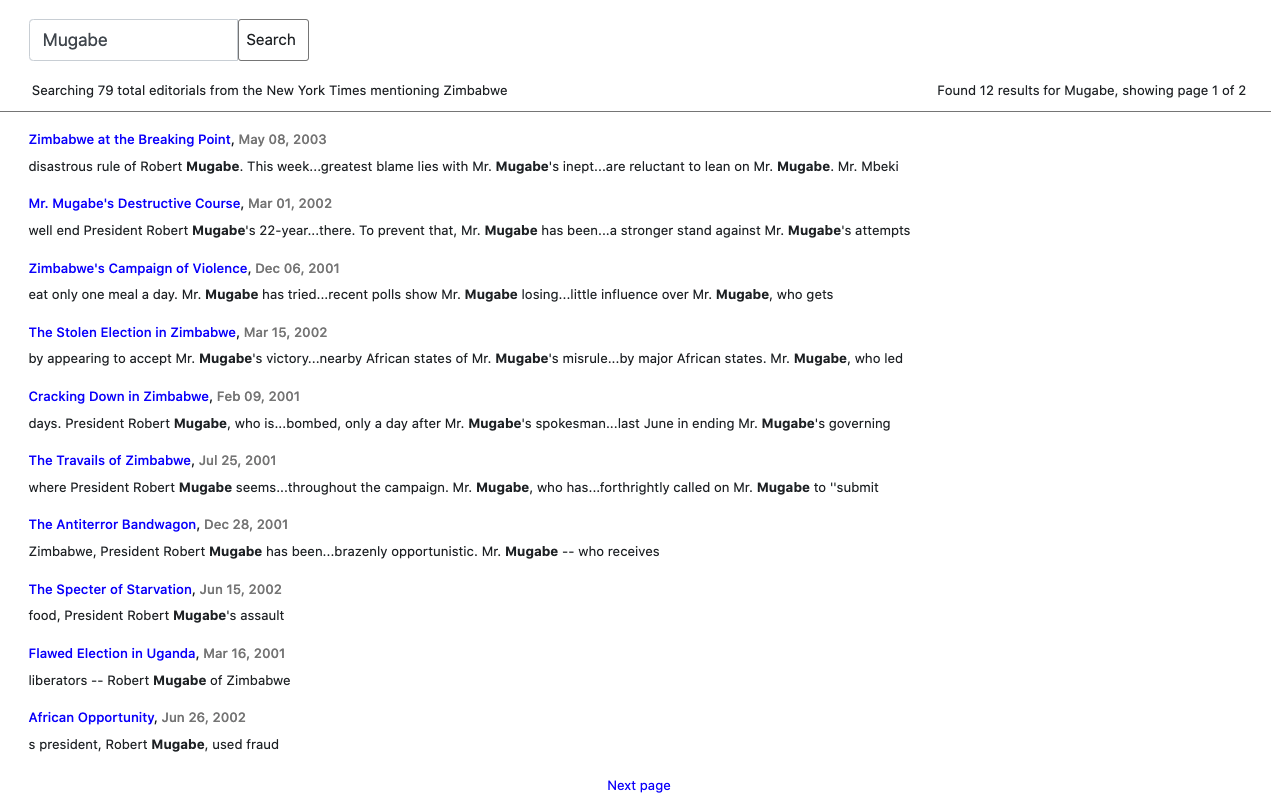
\includegraphics[width=1.0\linewidth]{figures/Appendix_ir.png}}
\caption{The IR baseline interface in our crowd study}
\label{f:appendix_ir_serp}
\end{figure}


\begin{figure}[t!]
\centering
\fbox{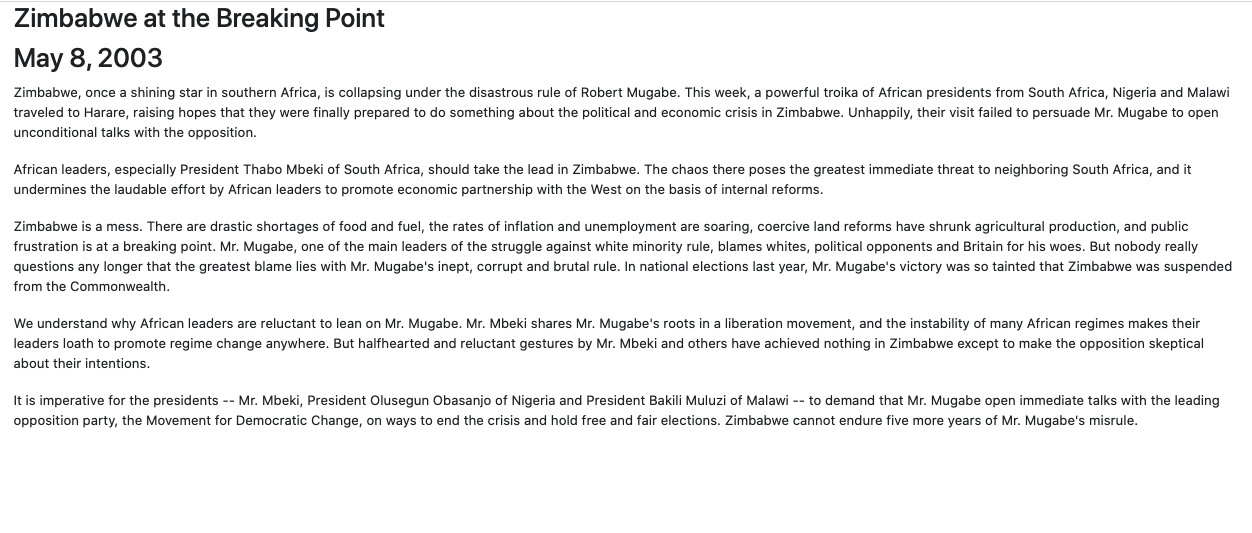
\includegraphics[width=1.0\linewidth]{figures/Appendix_ir_doc.png}}
\caption{A single search result from the IR interface in our crowd study}
\label{f:appendix_ir}
\end{figure}


\clearpage


\begin{figure}[t!]
\centering
\fbox{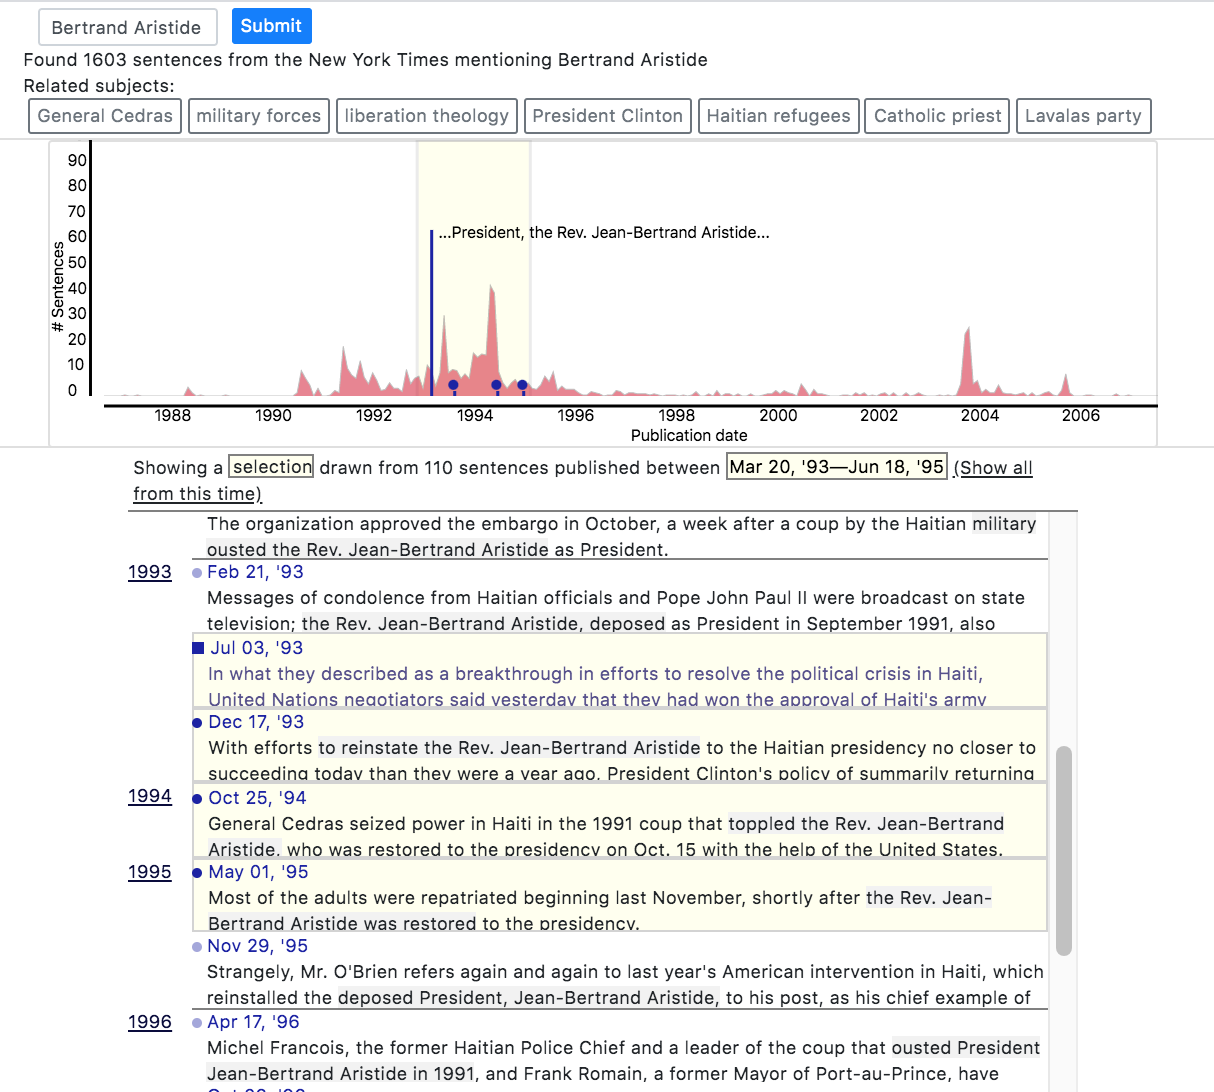
\includegraphics[width=.55\linewidth]{figures/p1.png}}
  \caption[Another early prototype of \ours]{
An early prototype of \ours, which used traditional, optimization-based text summarization methods from natural language processing \cite{McDonald} to try and select the most salient information from a given time period for display. This prototype selects four most ``important'' articles (shaded in light yellow in the feed below), to summarize the hundreds of articles mentioning the query ``Bertrand Aristide'' in \textit{The New York Times} from May 20, '93 to June 18, '95 (shown shaded in light yellow in the time series above).
\ifive~strongly disliked this approach, prompting a shift towards interfaces emphasizing transparency and trustworthiness. 
\textit{``I need to know what is included and why,''} \ifive~ explained. \textit{``I need to know why it is showing this limited view.''} \ifive~continued, \textit{``I am wary of algorithms that choose for me what the important facts are. I am a PhD historian. Leaving stuff out. We are taught to be critical of that.''} Ultimately, \ifive~noted, \textit{``History is written by the victors. What actually matters is what people choose to put in the timeline.''} We theorize that \ifive~could not trust the prototype because it seemed to lack the capacity to select important facts or the integrity to adhere to historical research principles; prior work in HCI (e.g.\ SMILY \cite{smiley}) assumes that in order to earn user trust, a system must both have the capacity to help the user and the integrity to adhere to principles which are important in a given domain.
}\label{f:prototype1}
\end{figure}


\begin{figure}[t!]
\centering
\fbox{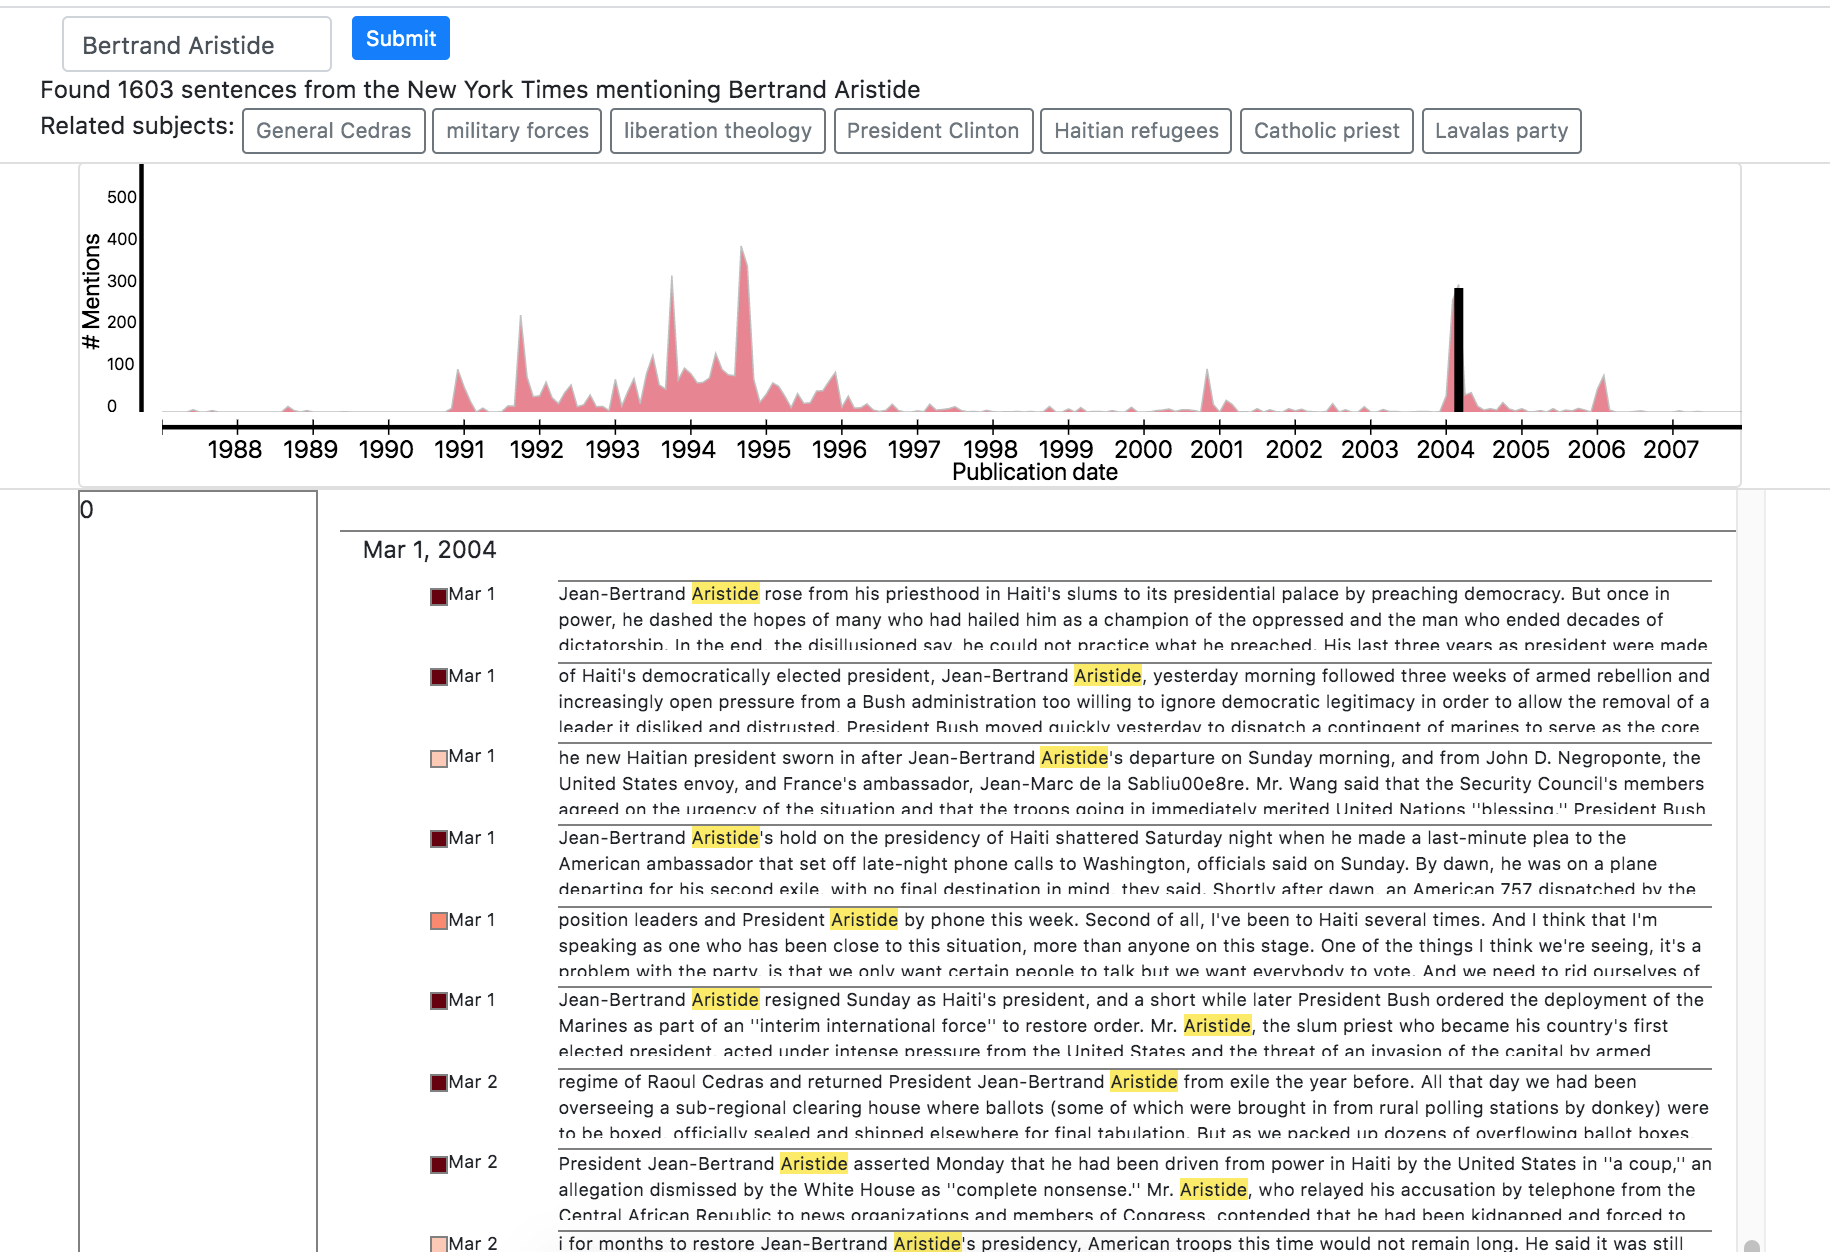
\includegraphics[width=.55\linewidth]{figures/p2.png}}
  \caption[An early prototype of \ours]{  
  An early prototype of \ours, displaying and highlighting every single mention of the query term ``Aristide'' in \textit{New York Times} articles mentioning ``Haiti''. ``Are we showing too much information in this interface?'' one researcher from our group asked \ifour, when presenting the prototype. ``This is literally every mention of your query term.''
\textit{``No this is good},''  \ifour~explained, \textit{``because of what I was calling the type II error concern [i.e.\ the fear of missing relevant material]. When I see something that is trying to decide or curate for me that is a worry. That is a red flag.''} 
However, \ifour~went on to explain how the interface needed to provide more context and transparency surrounding highlighted snippets. 
\textit{``With this design you have to click or read each snippet to see if it is relevant,''} he said.  ``\textit{The snippets are valuable and good but very small and you have to look at the contents of the article. Sometimes you can eliminate that by just quickly scanning the article title ... there needs to be a way to provide the information in a more transparent way.}'' 
(The search bar shown at the top is non-functioning mockup; the ``0'' on the left hand side is a placeholder.)
}\label{f:prototype2}
\end{figure}


\clearpage
\subsection{Additional Tables}
{
\begin{table}[h]
% \footnotesize % uncomment for thesis
% \centering % uncomment for thesis
\begin{tabular}{lccccc}
\toprule
ID     & Research experience & Library experience  & University role                & \multicolumn{1}{c}{Gender} & Topic     \\  \midrule
{P1} & 6                   & 0                  & PhD candidate                & Male                       & Iraq      \\
P2 & 5                   & 0                  & PhD candidate                & Male                       & Zimbabwe  \\
P3 & 4                   & 0                  & PhD candidate                & Female                     & combat    \\
P4 & 20                  & 0                  & Instructor/researcher        & Female                     & wages     \\
P5 & 0                   & 3                  & History librarian & Male                       & copyright \\ \bottomrule 
\end{tabular}
\caption[Participants in the interview study]{Interview study participants. We report history and library experience in years.}\label{t:particpants}
\end{table}
} %moved to appendix to save space
{
\begin{table}[h]
% \footnotesize %uncomment_for_thesis 
% \centering %uncomment_for_thesis
\begin{tabular}{@{}lccccc@{}}
\toprule
ID     & Research experience & Library experience & Academic role   & \multicolumn{1}{c}{Gender} & Research area     \\ \midrule
\rhone     & 5                   & 0                  & PhD student     & Male                       & Media and society \\
\rhtwo & 25                  & 0                  & Tenured faculty & Female                     & Space exploration \\ \bottomrule

\end{tabular}
\caption[Historians in the field study]{Historians in the field study. History and library experience are listed in years.}\label{t:field_study_particpants}
\end{table}
} % moved to appendix to save space
{
\begin{table}[h]
% \footnotesize %uncomment_for_thesis 
% \centering %uncomment_for_thesis 
\begin{tabular}{rccccc}
\toprule
    ID        & {Research experience} & {Library experience }   & {University role}   & {Gender}    &  {Field}   \\  \midrule
{I1} & 5-10  &  1-5    & PhD Candidate & Male & History \\
{I2} & 0 &  20-30  & Librarian & Female & Lib.\ Science \\ 
{I3} & 10-20   &  0      &  Junior Faculty  &   Female & Am.\ Studies \\
{I4} & 10-20 & 10-20 & Archivist & Male & Lib.\ Science  \\
{I5} & 10-20 & 10-20 & Librarian & Non-binary   & History  \\  \bottomrule
\end{tabular}
\caption[Interviewees in the needfinding study]{Interviewees in our needfinding study. We list research experience and library experience as a range of years. 
%%%(a range, in years), current university role, gender and field (based on highest post-graduate degree) of each interviewee. 
%%%I1 and I5 have experience both as librarians and as researchers. I4 conducts historical research during his work as an archivist. 
We abbreviate American Studies as Am.\ Studies and Library Science as Lib.\ Science.
}\label{t:interviewees}
\end{table}
}
%%Duff and Johnson = 11 interviews
%%Dalton + Charnigo = 278 historians
%%Chassanoff = 86 historians
%%Allen = 8 
%%Case
%%Duff, Craig, Cherry 581

\begin{table}[h]
% \small % uncomment for thesis
% \centering % uncomment for thesis
\begin{tabular}{@{}llcc@{}}
\toprule
Author(s) & Venue &  Study type & Participants  \\ \midrule
Allen and Sieczkiewicz \cite{allen}     &   \textit{Proc. ASIS\&T} (Info. Science)  &        Interview      &       8     \\
Case \cite{Case}     &  \textit{The Library Quarterly }   &     Interview         &     20       \\
Duff and Johnson     \cite{DuffJohnson}   &   \textit{The Library Quarterly}    &     Interview         &  10  \\     \midrule
Chassanoff \cite{Chassanoff}     &   \textit{The American Archivist}    &  Survey  &  86      \\
Dalton and Charnigo \cite{DaltonCharnigo}      &   \textit{College \& Research Libraries}    &   Survey           &     278       \\ 
Duff, Craig, and Cherry  \cite{DuffCraigCherry}      &   \textit{The Public Historian}    &    Survey         &    600         \\ \bottomrule
\end{tabular}\caption[A selection from prior work in library science and information science]{A selection from prior work in library science and information science, focused on the information-seeking behavior of historians.
These papers describe studies of $N=1002$ historians (in total).}\label{t:libraryscience}
\end{table}

%%%%Duff, Craig, and Cherry said both N=581 and N=585 in a table, which is a little confusing. in text they say 600 respondents %moved to appendix to save space

\clearpage
\bibliography{sample-base}
\bibliographystyle{ACM-Reference-Format}

\end{document}